\chapter{Contextualització}

\label{Contextualitzacio}

Abans d'entrar a definir quines seran les tasque si objectius específics d'aquest projecte, plantegem una breu aproximació al context del projecte, analitzant l'estat de l'art de l'àrea d'estudi.

%----------------------------------------------------------------------------------------
%	SECTION 2
%----------------------------------------------------------------------------------------

\section{Estat de l'art}

Per tal de plantejar les necessitats i projeccions del treball, així com les vies de desenvolupament del projecte, és necessari conèixer quina és la situació del monitoratge autoadaptatiu de sistemes software en la recerca actual.\\

En primer lloc, cal conéixer l’entorn referent als sistemes software autoadaptatius: és a dir, aquells que seran l’objectiu de monitoratge del nostre sistema de monitoratge (que no deixa de ser un altre sistema software autoadaptatiu). És interessant veure com la recerca i la investigació planteja, de forma pràcticament correlacionada, els conceptes de sistema autoadaptatiu i monitoratge.\\

\begin{figure}
\centering
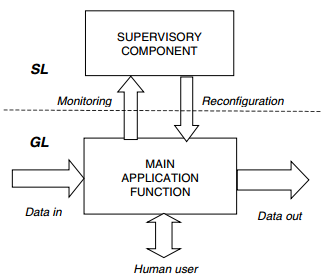
\includegraphics[width=8cm]{Figures/Figure1}
\decoRule
\caption[Arquitectura de sistemes auotadaptables monitorats]{Arquitectura de sistemes autoadaptables monitorats}
\label{fig:Figura1}
\end{figure}

De fet, documents de caràcter acadèmic tals com \cite{nashville} plantegen una arquitectura d’autoadaptabilitat per sistemes software basada en la supervisió o monitoratge. Tal com podem veure a la figura ~\ref{fig:Figura1}, destaquem dos components principals: l’aplicació principal, o \textbf{Main Application Function}, equivalent al sistema software (servei web, aplicació mòbil, etc.) encarregat d'una funcionalitat específica i sobre el qual volem realitzar el control de qualitat; i el component supervisor, o \textbf{Supervisory Component}, que s'encarrega d'executar aquest control de qualitat.\\

La interacció i arquitectura plantejada en la figura és relativament senzilla. El component software a avaluar forma part del domini del sistema a avaluar (\textit{ground-level}, GL). En la seva activitat, aquesta aplicació o sistema rep una sèrie de dades (que dependrà de la naturalesa i objectiu del sistema), i produeix uns resultats en base a aquest \textit{input}. Paral·lelament, com qualsevol sistema orientat a l'ús, existeix una interacció sistema-usuari. Més enllà del domini i les característiques pròpies dels sistemes software, es presenta l'entorn corresponent al sistema de supervisió o monitoratge (\textit{supervisory-level}, SL). En aquest nivell trobem des d'un punt de vista lògic el component de supervisió o monitor, que interacciona amb l'aplicació principal de dues formes diferents:

\begin{itemize}
\item \textbf{Monitoratge}. Procés d'interacció entre el component principal i el monitor on el primer envia informació al segon. L'aplicatiu produeix, com a conseqüència de la seva activitat, informació i dades que envia com a \textit{output} al monitor. Aquesta informació ha d'estar prèviament definida i estructurada, de tal manera que el monitor sigui capaç d'interpretar-la.
\item \textbf{Reconfiguració}. El monitor procesa les dades que rep com a input del monitoratge i, segons els criteris d'adaptabilitat establerts, aplica els canvis o reconfiguracions pertinents en el sistema software monitorat. D'aquesta manera, la lògica encarregada d'interpretar la informació i prendre decisions d'adaptabilitat (SL) queda totalment separada de la lògica del domini de l'aplicatiu (GL).
\end{itemize}

Partint d'aquest punt, aquest document estableix les premisses del monitoratge i les necessitats de reconfiguració d’aquests tercers sistemes softwares, la naturalesa dels quals és diversa i heterogènia. Noti's que, de fet, l'anterior disseny presenta una arquitectura genèrica aplicable a qualsevol entorn software, independentment de la naturalesa del domini monitorat. Tot i així, existeix una àmplia recerca especialitzada: publicacions com \cite{napols} es centren en analitzar els requisits, necessitats i funcions principals del monitoratge i reconfiguració de sistemes i recursos al núvol (p.e. serveis web).\\

La documentació i bibliografia referent als sistemes software autoadaptables i als sistemes de supervisió i monitoratge és molt àmplia. Tot i així, si focalitzem la recerca a la problemàtica a resoldre, és a dir, l’autoadaptabilitat i reconfiguració dels sistemes de monitoratge, no trobem un treball tan profunditzat i específic com en el cas prèviament explicat.\\

En alguns documents, com per exemple el ja esmentat \cite{napols}, es mencionen criteris del disseny de la capa de supervisió, entre els quals entren en joc, p.e., factors com la previsió d’errors a la capa de l’aplicatiu principal, o ve esdeveniments/disparadors inesperats. I, com és lògic, una reacció i canvis per part del sistema de monitoratge. Aquest plantejament es fa des del punt de vista dels sistemes software monitorats, però no des del punt de vista dels propis sistemes de monitoratge. En el nostre cas, caldrà plantejar-nos com podem fer que el nostre sistema sigui el més flexible i adaptable en temps real possible. I, addicional, com podem dissenyar el sistema per tal de disposar en tot moment de dades reals sobre l'execució i el comportament d'aquest.\\

En altres documents, tals com \cite{ibm}, es defineixen models autònoms d’autoadaptabilitat i reconfiguració autònoma, basats en tècniques de detecció d’esdeveniments i canvis en el propi sistema. Conceptes com l’anàlisi de l’estat del sistema, el monitoratge i l’execució d’una reconfiguració entren en joc dins d’aquest pla. El concepte de "reconfiguració" serà un dels principals que tractarem en el nostre projecte, entenent-la com la modificació en temps real d'un procés de monitoratge d'un monitor, amb l'objectiu de millorar la seva activitat de control de qualitat.\\

Una aproximació interessant és analitzada i desenvolupada a \cite{heterogeneous}. En aquesta publicació es treballen a fons 2 aspectes principals. Per una banda, la necessitat de concebre el monitoratge des d'un punt de vista heterogeni per tal que l'estudi i les propostes en aquest àmbit puguin ser reaprofitables el màxim possible. Però un segon aspecte interessant es tracta en aquest document: la modelació, mitjançant llenguatge formalitzat, de les directives d'adaptacions dels sistemes de monitoratge. En concret, es planteja utilitzar regles de monitoratge basades en llenguatge OCL (\textit{Object Constraint Language}). La premisa és senzilla: mitjançant la formalització de regles o directives que es puguin gestionar de forma dinàmica, el sistema és capaç de reaccionar de forma automàtica a les violacions de certes restriccions d'integritat, per tal d'accionar de forma completament autònoma i reconfigurar el monitoratge (o els sistemes softwares monitorats) sota aquests criteris).\\

Davant els conceptes presentats en aquests treballs, sorgeix la pregunta: com es pot presentar una proposta que suposi una millora, o si més no un avenç, respecte l'estat de l'art actual? El propòsit d'aquest TFG és unificar els punts forts de diversos d'aquests projectes o recerques per realitzar una proposta unificada que satisfaci tots els criteris òptims destacats anteriorment. Aquests punts inclouen:

\begin{itemize}
\item El disseny i implementació d'un sistema composat per \textbf{dos subsistemes integrats}: un sistema de monitoratge i un sistema d'adaptabilitat, on el segon actuï sobre el primer
\item El plantejament d'una proposta de disseny prou àmplia com per poder garantir la seva \textbf{heterogeneïtat}, independentment d'aspectes relacionats als monitors com la tecnologia o l'àrea monitorada
\item El disseny i implementació de components de forma totalment distribuïda i independentment, aportant no només flexibilitat i desacoblament en el desplegament físic, sinó també llibertat de reaprofitament i extensió del sistema
\item La proposta d'un sistema de gestió de l'adaptabilitat mitjançant un llenguatge formal, que vagi més enllà de la modelació de directives de canvi proposada a \cite{heterogeneous} i permeti un control màxim del sistema, del seu estat actual, i la gestió de diferents propostes de reconfiguració més personalitzables
\end{itemize}

A tot això, cal afegir la importància de destacar que aquest projecte, si bé té per objectiu la generació d'un producte final aplicable i reutilitzable per altres components, està especialment orientat a la recerca i a ser en sí mateix una proposta d'aproximacions diverses a la resolució de diversos problemes. Per tant, per a què suposi encara un impacte major en l'estat de l'art de la temàtica, tots els components i documentació generats seran publicats sota llicències de software lliure, amb l'objectiu que aquests puguin ser explotats i desenvolupats en treball futur, ja sigui sota responsabilitat del propi autor com per altres desenvolupadors.

%-----------------------------------
%	SUBSECTION 2
%-----------------------------------

\section{Projecte SUPERSEDE}

Com a part de l'estat de l'art i punt de partida pel desenvolupament del sistema, cal introduïr el projecte SUPERSEDE\cite{supersede}. Aquest projecte forma part del \textit{Horizon 2020 Programme}\cite{horizon}, un programa de recerca i innovació financiat i gestionat per la Unió Europea. Actualment, compta amb la participació de diverses empreses, fundacions i universitats, entre les quals s'inclou la pròpia UPC. \\

Aquest projecte planteja una proposta del cicle de vida i la gestió dels serveis software i les aplicacions, amb l'objectiu final similar al plantejat com a premisa d'aquest Treball de Final de Grau: millorar la qualitat de l'execució dels sistemes software i, en conseqüencia, l'experiència de l'usuari final en l'interacció amb aquests sistemes. \\

Dins aquest cicle de vida, orientat al control de qualitat dels sitemes software, es proposen 4 fases:

\begin{enumerate}
\item \textbf{Col·lecció}. L'obtenció i emmagatzematge de dades que puguin resultar d'interès pel control de qualitat. La naturalesa d'aquestes dades (així com el format i altres criteris) dependran de l'objectiu d'aquest anàlisi i el tipus de dades tractat. Així, aquestes poden incloure des de dades purament analítiques (p.e. \% de disponibilitat del sistema) o bé contextuals (p.e. missatges o continguts introduïts al sistema).
\item \textbf{Anàlisi}. Les dades obtingudes en la fase anterior tenen un significat, una informació que el sistema ha de ser capaç d'extreure i comprendre. En aquesta fase, les dades es transformen en coneixement en relació a l'estat del sistema, a través de diverses tècniques analítiques, de nou en funció del marc d'estudi i el context. Per exemple, es podrien valorar tècniques d'anàlisi de llenguatge natural per estudiar les valoracions d'usuaris introduïdes a un sistema.
\item \textbf{Decisió}. El coneixement produït a l'anterior fase genera la capacitat de prendre decisions de millora i actuació sobre el sistema software. És a dir, deriva en una o vàries propostes d'adaptació. Les eines de presa de decisions entren en joc en aquesta fase, rebent com a entrada la informació i, a partir dels criteris i paràmetres definits en relació a aquesta informació, es produeix la proposta d'adaptació del sistema.
\item \textbf{Adaptació}. Un cop el sistema ha estat capaç de produir de forma automàtica una proposta de millora o adaptació del sistema, aquesta s'aplica sobre el component monitorat amb l'objectiu de millorar l'experiència de l'usuari. Arribats a aquest punt, es tanca el cicle de control de qualitat, reflectint la transformació de l'input de la fase de col·lecció, les dades, fins a l'output d'aquesta darrera fase, l'adaptació del sistema.
\end{enumerate}

\begin{figure}
\centering
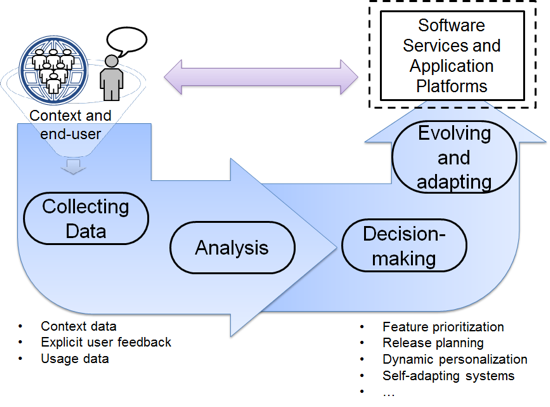
\includegraphics[width=10cm]{Figures/Figure2}
\decoRule
\caption[Cicle de vida i entorn proposat per SUPERSEDE]{Cicle de vida i entorn proposat per SUPERSEDE}
\label{fig:Figura2}
\end{figure}

La figura ~\ref{fig:Figura2} resumeix aquest cicle de vida i les característiques del context de les seves fases. Tal i com es pot observar, la principal font de dades amb les quals aquest control de qualitat es nodreix es l'experiència de l'usuari final, el context on s'executa aquesta aplicació o sistema i les dades generades del propi ús i funcionament del sistema. És, per tant, un aspecte clau l'obtenció de \textbf{dades en execució real}, que seran les que ens permetin aplicar aquest cicle regularment. Regularitat que serà crucial per satisfer l'objectiu d'anàlisi de la qualitat del sistema: només amb dades actuals i constants serem capaços de conèixer l'activitat real del nostre sistema i actuar en conseqüència.\\

Aquest cicle de vida no és més que una descripció del cicle \textit{MAPE-k} \cite{mapek1}\cite{mapek2}, un cicle de vida del software orientat a la retroalimentació i adaptació de l'activitat classificat en aquestes quatre fases: \textit{\textbf{M}onitoring}, \textit{\textbf{A}nalysis}, \textit{\textbf{P}lan} i \textit{\textbf{E}nactment}.\\

En aquest context identifiquem per tant 4 sectors o subsistemes amb un objectiu específic que, integrats, serveixen a un propòsit genèric. Si ens plantegem com encaixa aquest model dins el nostre tema d'estudi (és a dir, l'adaptabilitat dels sistemes de monitoratge) podem establir una relació directa amb les fases de \textbf{col·lecció} de dades i \textbf{adaptació}. Dins aquesta primera fase de col·lecció, necessitem definir un sistema capaç d'obtenir aquestes dades, en funció dels sistemes a controlar i de l'interès que tinguem sobre aquests sistemes. Aquest sistema de \textbf{monitoratge} estarà compost per un conjunt definit de monitors, encarregats de recollir aquesta informació. Per altra banda, si volem dotar a aquest sistema de monitoratge d'adaptabilitat, i per tant, garantir un control de qualitat sobre aquests monitors, necessitem establir un sistema que gestioni l'activitat dels monitors i defineixi adaptacions a aplicar sobre aquests monitors.\\

Pel desenvolupament d'aquest projecte, ens centrarem en aquestes dues parts: el sistema encarregat de la fase de col·lecció de dades (monitors), i el sistema encarregat de gestionar i aplicar les adaptacions sobre aquest sistema de col·lecció. De la mateixa manera, es treballa la integració entre aquests dos components, per generar com a resultat final l'objectiu d'aquest projecte: un sistema de monitoratge autoadaptable, heterogeni i distribuït.